\documentclass[english,notitlepage]{revtex4-1}  % defines the basic parameters of the document
%For preview: skriv i terminal: latexmk -pdf -pvc filnavn



% if you want a single-column, remove reprint

% allows special characters (including æøå)
\usepackage[utf8]{inputenc}
%\usepackage[english]{babel}

%% note that you may need to download some of these packages manually, it depends on your setup.
%% I recommend downloading TeXMaker, because it includes a large library of the most common packages.

\usepackage{physics,amssymb}  % mathematical symbols (physics imports amsmath)
\include{amsmath}
\usepackage{graphicx}         % include graphics such as plots
\usepackage{xcolor}           % set colors
\usepackage{hyperref}         % automagic cross-referencing (this is GODLIKE)
\usepackage{subcaption}
\usepackage{listings}         % display code
\usepackage{float}
\usepackage{enumitem}
%\usepackage[section]{placeins}
\usepackage{algorithm}
\usepackage[noend]{algpseudocode}
\usepackage{tikz}
\usetikzlibrary{quantikz}
% defines the color of hyperref objects
% Blending two colors:  blue!80!black  =  80% blue and 20% black
\hypersetup{ % this is just my personal choice, feel free to change things
    colorlinks,
    linkcolor={red!50!black},
    citecolor={blue!50!black},
    urlcolor={blue!80!black}}

%% Defines the style of the programming listing
%% This is actually my personal template, go ahead and change stuff if you want



%% USEFUL LINKS:
%%
%%   UiO LaTeX guides:        https://www.mn.uio.no/ifi/tjenester/it/hjelp/latex/
%%   mathematics:             https://en.wikibooks.org/wiki/LaTeX/Mathematics

%%   PHYSICS !                https://mirror.hmc.edu/ctan/macros/latex/contrib/physics/physics.pdf

%%   the basics of Tikz:       https://en.wikibooks.org/wiki/LaTeX/PGF/Tikz
%%   all the colors!:          https://en.wikibooks.org/wiki/LaTeX/Colors
%%   how to draw tables:       https://en.wikibooks.org/wiki/LaTeX/Tables
%%   code listing styles:      https://en.wikibooks.org/wiki/LaTeX/Source_Code_Listings
%%   \includegraphics          https://en.wikibooks.org/wiki/LaTeX/Importing_Graphics
%%   learn more about figures  https://en.wikibooks.org/wiki/LaTeX/Floats,_Figures_and_Captions
%%   automagic bibliography:   https://en.wikibooks.org/wiki/LaTeX/Bibliography_Management  (this one is kinda difficult the first time)
%%   REVTeX Guide:             http://www.physics.csbsju.edu/370/papers/Journal_Style_Manuals/auguide4-1.pdf
%%
%%   (this document is of class "revtex4-1", the REVTeX Guide explains how the class works)


%% CREATING THE .pdf FILE USING LINUX IN THE TERMINAL
%%
%% [terminal]$ pdflatex template.tex
%%
%% Run the command twice, always.
%% If you want to use \footnote, you need to run these commands (IN THIS SPECIFIC ORDER)
%%
%% [terminal]$ pdflatex template.tex
%% [terminal]$ bibtex template
%% [terminal]$ pdflatex template.tex
%% [terminal]$ pdflatex template.tex
%%
%% Don't ask me why, I don't know.

\begin{document}

\title{Project 1}      % self-explanatory
\author{Alessio Canclini, Filip von der Lippe}          % self-explanatory
\date{\today}                             % self-explanatory
\noaffiliation                            % ignore this, but keep it.


\maketitle

\textit{List a link to your github repository here!}

\section*{Problem 1}
\begin{align}
  - \frac{d^2u}{dx^2} = f(x)
  \label{eq:poisson}
\end{align}

\begin{itemize}
  \item source term: $f(x) = 100e^{-10x}$
  \item $x$ range $x \in [0,1]$
  \item boundary conditions: $u(0) = 0$ and $u(1) = 0$
\end{itemize}

\begin{align}
  u(x) = 1 - (1 - e^{-10})x- e^{-10x}
  \label{eq:u(x)}
\end{align}
Checking analytically that an exact solution to Eq. \ref{eq:poisson} is given by Eq. \ref{eq:u(x)}.

\begin{align*}
  \frac{du}{dx} & = 1 - e^{-10} + 10e^{-10x} \\
  \frac{d^2u}{dx^2} & = -100e^{-10x} \\
  -\frac{d^2u}{dx^2} & = 100e^{-10x} \\
  -\frac{d^2u}{dx^2} & = f(x)
\end{align*}

\section*{Problem 2}
\begin{figure}[H]
  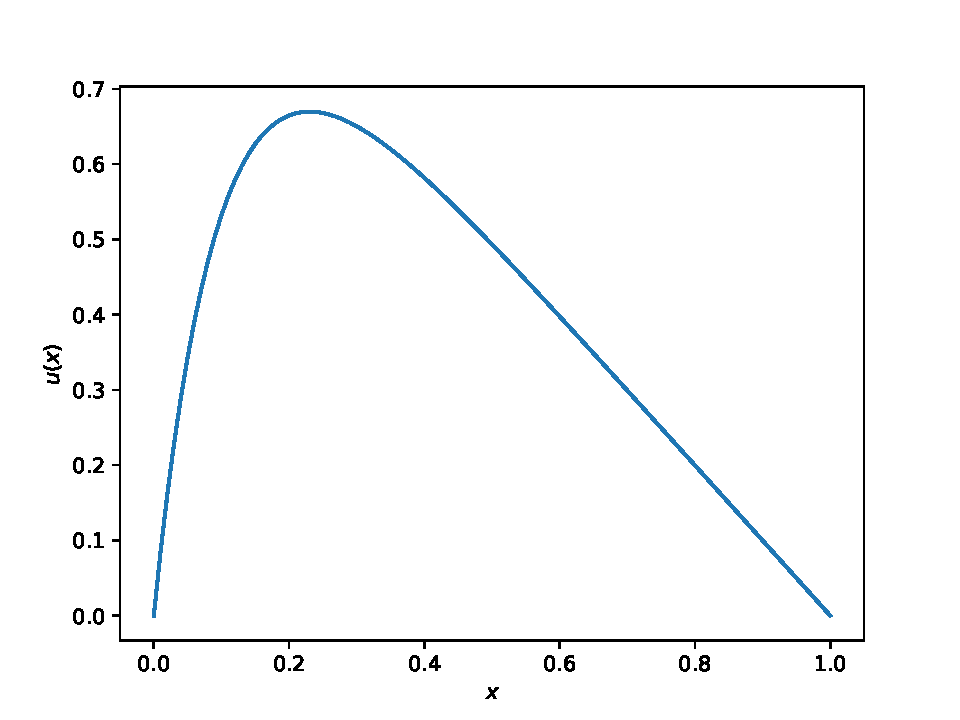
\includegraphics{../figures/x_u_plot.pdf}
  \caption{Plot of $u(x)$.}
  \label{fig:x_u}
\end{figure}

\section*{Problem 3}
By using the taylor approximation of the second derivative we can discretize the second derivative in the Poission equation:
\begin{align*}
  \frac{\partial^2 u }{\partial x^2} \approx \frac{u_{i+1} - 2 u_i + u_{i-1}}{h^2} + O(h^2)
\end{align*}
Here we have the stepsize $h$ and the truncation error $O$. The one-dimensional Poisson equation can then be written for the approximated version of $u$ as $v$ like:
\begin{align}
    -\frac{v_{i+1} - 2 v_i + v_{i-1}}{h^2} = f_i
    \label{eq:poiss_disc}
\end{align}

\section*{Problem 4}
We can rewrite the discretized equation as a matrix equation for $n+1$ number of points and $n-1$ unknown points ($v_0$ and $v_n$ are known) with the $n-1\times n-1$ matrix $\boldsymbol{A}$. We rewrite the discretized Poisson funcion:
\begin{align*}
  2 v_1- v_2 &= f_1 h^2\\
  -v_{1} +2 v_2 - v_{3} &= f_2 h^2 \\
    \vdots \\
  -v_{n-3} + 2 v_{n-2} - v_{n-1} &= f_{n-2} h^2\\
  - v_{n-2} + 2 v_{n-1}  &= f_{n-1} h^2
\end{align*}
This can be written in terms of the following matrix equation where we rewrite $f_i h^2$ for $i = 1,2,\dots n-1$ as $g_i$
\begin{align*}
  \begin{bmatrix}
    2 & -1 & 0 & 0 & \dots &0 \\
    -1 & 2 & -1 & 0 &\dots& 0 \\
    \vdots & \vdots & \vdots & \vdots & \ddots & \vdots\\
    0 & 0 & \dots & -1 & 2 & -1 \\
    0 & 0 & \dots & \ 0 &-1 & 2
  \end{bmatrix}
  \begin{bmatrix}
    v_1 \\
    v_2 \\
    \vdots\\
    v_{n-2}\\
    v_{n-1}
  \end{bmatrix}
  =
  \begin{bmatrix}
    g_1 \\
    g_2 \\
    \vdots\\
    g_{n-2}\\
    g_{n-1}
  \end{bmatrix}
\end{align*}
\section*{Problem 5}

\begin{enumerate}[label= \alph*)]
  \item Since the vector $\vec{v*}$ of length $m$ represents a complete solution of the descretized Poisson equation it contains all values in $\vec{v}$ in addition to the boundary conditions. The relation bethween $n$ and $m$ is therfore $m=n+2$.
  \item Solving $\boldsymbol{A}\vec{v} = \vec{g}$ for $\vec{v}$ gives us all but the first an last value in $\vec{v*}$. So all but the boundary values.
\end{enumerate}

\section*{Problem 6}
\begin{enumerate}[label= \alph*)]
  \item We can use the Thomas algorithm to row reduce the matrix $\boldsymbol{A}$ to give us a solution of the equation $\boldsymbol{A} \vec{v} = \vec{g}$. This is done in two steps. We first define the three diagonals as three vectors. The sub diagonal $\vec{a}$ the diagonal $\vec{b}$ and the superdiagonal $\vec{c}$ where the $i$ element in theese vectors corresponds to the $i$ row of the matrix $\boldsymbol{A}$. We define $n$ unknowns and the matrix $\boldsymbol{A}$ as $n\times n$
  \begin{enumerate}[label=\roman*)]
    \item The first step is forwards substitution. We define a numer $w$ for each step and overwrite the $i$ element of both $b$ and $g$ starting at index 2. This means overwrite the values in the original vectors $b$ and $g$, but at the same time we dont have to define new vectors to store new values. For large $n$ this will reduce both the computation time and memory usage for the data machine\\\\
    $\text{for }i=2,..,n$:
    \begin{align*}
      w &= \frac{a_i}{b_{i-1}} \\
      b_i &= b_i - wc_{i-1} \\
      g_i &= g_i - wg_{i-1}
    \end{align*}
    \item The second and last step is back substitution where we find an expression for $\vec{v}$. We start at our last element and work our way backwards:
    \begin{align*}
      v_n &= \frac{g_n}{b_n} \\
      v_i &= \frac{g_i - c_i v_ {i+1}}{b_i} \quad \text{for } i = n-1,...,1
    \end{align*}
  \end{enumerate}
  \item We find the number of FLOPs for this algorithm by counting the number of floating point operations the computer has to do. For the first step we have 3 FLOPs (1 subtraction 1 division and one multiplication) for defining $b_i$ and  $g_i$ each. Since we loop this operation $n-1$ times we end up with a  totalt number of $6(n-1)$ FLOPs.

  For back substitution we have 1 FLOP calculating $v_n$, and three FLOPs calculating $v_i$ $n-1$ times. This gives us $3(n-1)+1$ FLOPs

  The total FLOPs of the general algorithm is $9n-8$
\end{enumerate}
\section*{Problem 7}
\section*{Problem 8}
\section*{Problem 9}
\begin{enumerate}[label= \alph*)]
  \item For the special case we dont need to do new computations for every $i$ element of the vectors $\vec{a}$ and $\vec{c}$ and thus don't need to assign and use these variabeles.
  \begin{enumerate}[label=\roman*)]
    \item The first step is forwards substitution. We have to define $b_1 = 2$ and then loop over the rest:
    \begin{align*}
      b_i &= b_i + \frac{1}{b_{i-1}} \quad  \text{for }i=2,..,n \quad\\
      g_i &= g_i + \frac{1}{b_{i-1}}g_{i-1} \quad  \text{for } i = 2,..,n \quad
    \end{align*}
    \item The second and last step is back substitution where we find an expression for $\vec{v}$. We start at our last element and work our way backwards:
    \begin{align*}
      v_n &= \frac{g_n}{b_n} \\
      v_i &= \frac{g_i + v_{i+1}}{b_i} \quad \text{for } i = n-1,...,1
    \end{align*}
  \end{enumerate}
  \item Since we know that $a,c = -1$ we are abel to reduce the amount of FLOPs compared to the general algorithm. For the forward substitution we have $2(n-1)$ FLOPs to compute $b_i$ and the same for $g_i$. The back substitution requires 1 FLOP for $v_n$ and $2(n-1)$ FLOPs for $v_i$. This gives us a total of $6n-5$ FLOPs for the special algorithm.
\end{enumerate}

\section*{Problem 10}
\begin{figure}[H]
  \begin{subfigure}{.5 \textwidth}
    \centering
    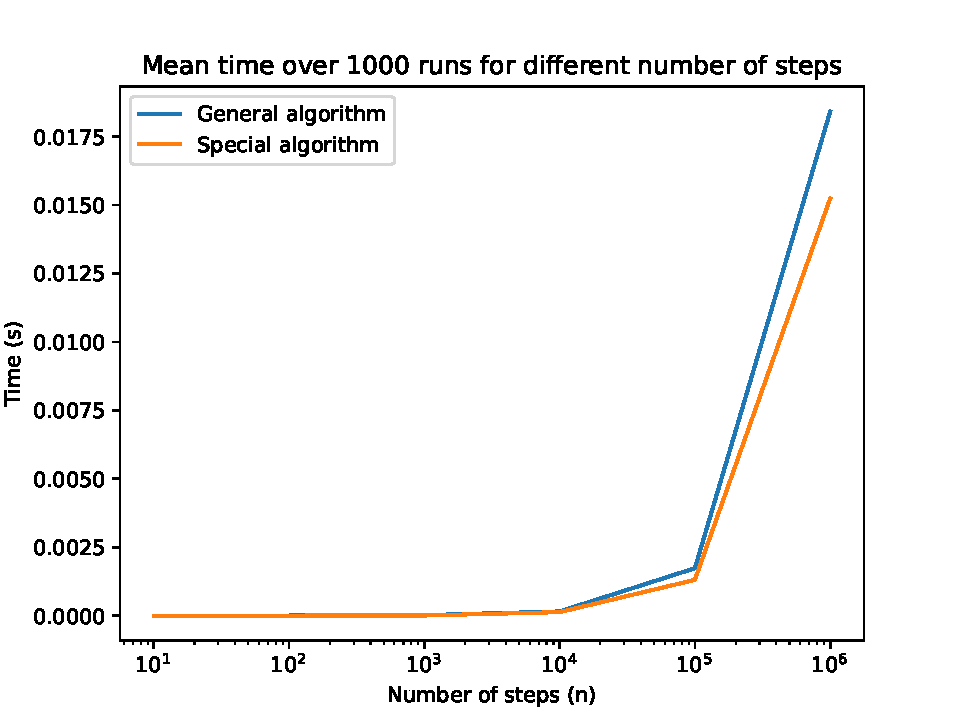
\includegraphics[width=\textwidth]{../figures/mean_time.pdf}
    \caption{}
    \label{fig:mean_time}
  \end{subfigure}
  \begin{subfigure}{.5 \textwidth}
    \centering
    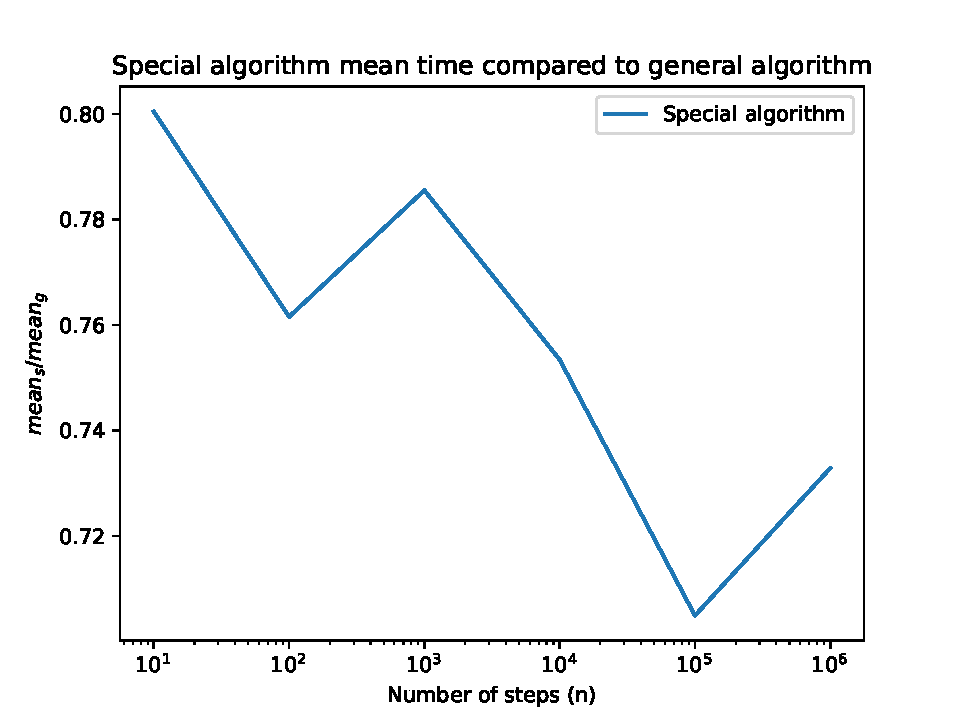
\includegraphics[width=\textwidth]{../figures/mean_time_rel.pdf}
    \caption{}
    \label{fig:mean_time_rel}
  \end{subfigure}
\end{figure}

\begin{figure}[H]
  \centering
  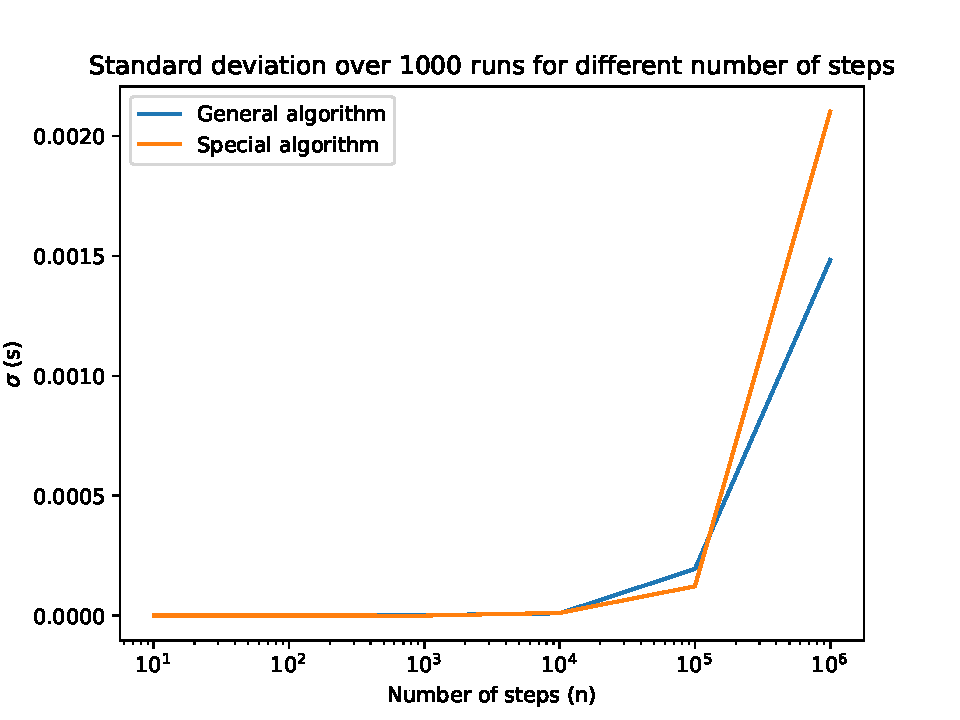
\includegraphics[width=.8\textwidth]{../figures/std_time.pdf}
  \caption{}
  \label{fig:std_time}
\end{figure}

\end{document}
